\subsection{Independent TCCON validation}
\label{sec:result-tccon_val}


%Use AK-harmonized TCCON as the primary reference and direct TCCON as a
%documented secondary comparison. Report the current production values only
%after regenerating the manuscript table from the frozen tag.

%The paragraph order should be:

1. one-sentence recap of the sample and coincidence criteria, citing
   Sect. 3.5;
2. mean absolute bias and footprint RMSE;
3. number of improved station-days;
4. Wilcoxon and site-clustered bootstrap results;
5. radius/window and QF0/QF1 sensitivity;
6. high-latitude and worsening cases.

Keep direct-reference results nearby but do not let the dual-reference
explanation obscure the AK-harmonized primary result.


After understanding the general performance of the \emph{DE} model in Sect.~\ref{sec:result-model_comp}, we then evaluate its correction capability compared to TCCON observations in detail. Again, all TCCON \xco are corrected following the description in Sect.~\ref{sec:method-eval-obs-xco2} to consider the difference in averaging kernels and prior profiles. The collocation search radius between the TCCON stations and the OCO-2 soundings is set to $100$~km, and the temporal search window to $\pm1$~h around the OCO-2 overpass. Note that these 75 station-days for 18 sites from December 2014 to December 2021 are chosen manually, as we want to have more available data for stations near the coastline, and we are unable to run all OCO-2 overpass cases.


Across all 75 station-days, the station-day mean absolute bias ($|$bias$|$) falls from 1.26$\pm$1.33 to 0.82$\pm$0.60 ppm and the per-footprint RMSE from 2.67 to 1.20 ppm (Fig.~\ref{fig:tccon_dumbbel}). The per-footprint RMSE improves in 71 of the 75 station-days, while the station-day mean bias improves in 46 of 75. The remaining 29 worsen only slightly, median $+0.28$ ppm, mostly from near-zero starting biases. The improvement is significant under a paired Wilcoxon test on station-day $|$bias$|$ (p = 0.0063, n = 75) and under site-clustered bootstrap intervals, with and without the high-latitude TCCON station Ny-Ålesund at 78.93$^\circ$N (Fig.~\ref{fig:tccon_significance_robustness}). The improvement holds at every collocation radius $\times$ window combination (25/50/100 km $\times$ $\pm$30/60/120 min), and it is largest at a tighter 50 km $\times$ $\pm$30 min window. This is expected, given that the correction is a spatially localized process. However, we use a larger search window to obtain more statistics and follow the $\pm1$~h window as in \citet{das2025oco2_v111_tccon_ggg2020}.

Additionally, we analyze QF=0 and QF=1 footprints separately (Fig.~\ref{app-fig:qf01_DE_eval}) and see that the $|$bias$|$ significantly decreases for QF=1 from 1.57$\pm$1.43 to 0.89$\pm$0.62, with the footprint RMSE reduced from 3.19 to 1.31. The $|$bias$|$ and footprint RMSE also improve for QF=0 but with smaller magnitudes. This is expected, as footprints with QF=0 have better retrieval quality and could be less influenced by clouds. We also see that the correction is larger when the station-mean nearest-cloud distance of OCO-2 footprints is small, confirming that our correction works in the right direction.

For all TCCON stations we used, Ny-Ålesund is the only station in our comparison poleward of 60$^\circ$ latitude, and high-latitude scenes are correspondingly rare in the training population. Only 5.3\,\% of the 17.8 million training
footprints lie poleward of $|60^\circ|$ (936,178) and 2.3 \% poleward of $|70^\circ|$ (411,649). Nevertheless, the ten Ny-Ålesund station-days receive the strongest corrections in the network. The station-day mean $|$bias$|$ falls from 2.18 to 1.31~ppm and the per-footprint RMSE from 4.74 to 1.95~ppm, both roughly twice the network-average improvement. The largest single correction of the comparison (from $-8.20$ to $-0.86$~ppm on 17 June 2017) occurs here. This is also why excluding
Ny-Ålesund reduces the magnitude of all three aggregate improvements in Fig.~\ref{fig:tccon_significance_robustness}a while their significance is retained ($p \le 0.016$). The headline result is not driven by this single site, but the site benefits from the correction more than any
other. At the same time, the corrected Ny-Ålesund residuals remain the largest in the network and are sign-consistent (positive in 7 of 10 station-days, up to $+2.9$~ppm), so a systematic high-latitude bias
survives the correction. We attribute this remaining bias to the thin training support poleward of 60$^\circ$ together with the extreme observation geometry (high solar zenith angle, seasonal snow and ice), and we regard the high-latitude regime as the part of the domain where the correction is least constrained. Additional high-latitude references (e.g., Sodankylä, East Trout Lake, Eureka) would be needed to validate it independently, and we return to this limit in Sect.~\ref{sec:limitation}.


The worsening cases are informative about the limits of the anomaly formulation rather than about the model fit. The bright-surface stratum (\ce{O2}A-band albedo $> 0.4$; 12{,}037 footprints, 11.4\,\% of the TCCON comparison set) shows the largest post-correction residual (1.55~ppm) and a worsened-footprint fraction of 0.50. This is not a prediction failure: on genuinely held-out dates in cross-validation, the model's anomaly skill is independent of albedo (residual RMSE 0.53--0.60~ppm and calibration $\langle z^2\rangle \approx 1.1$ across all albedo deciles), and even at TCCON the correction reduces the bright-surface footprint RMSE from 4.58 to 1.55~ppm. What remains after correction over bright scenes is a bias component that is nearly constant within an overpass. Such a common-mode component cancels in the within-orbit anomaly target by construction, so the model is never trained to remove it; the correction takes out the anomaly part and leaves the common-mode part behind. Because the remaining residual is then uncorrelated with the applied correction, the per-footprint worsened-or-improved count degenerates toward a coin flip (0.50, against 0.19--0.39 elsewhere), while the aggregate error still improves. The bright-surface stratum is therefore under-corrected rather than mis-corrected, in line with the high-AOD stratum, and both point to the same future extension: a complementary term for along-track common-mode bias, which the present per-footprint anomaly correction intentionally does not model.





\begin{figure}[t]
\centering
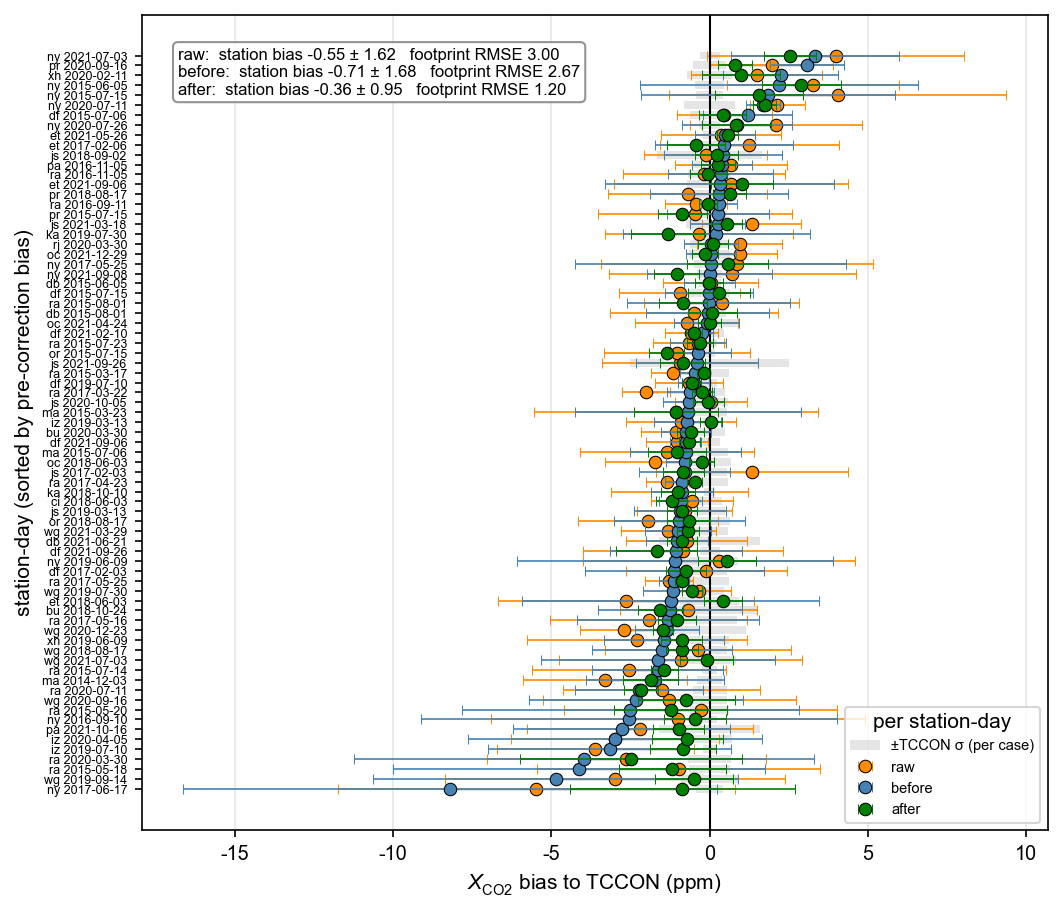
\includegraphics[width=0.8\textwidth]{figures/fig08_tccon_dumbbell.png}
\caption{Independent TCCON validation (AK-harmonised reference; before-vs-after differences are invariant to it): station-day mean bias before and after correction for all 75 station-days (18 sites, 2014–2021; r = 100 km, ±60 min).}
\label{fig:tccon_dumbbel}
\end{figure}



\begin{figure}[t]
\centering
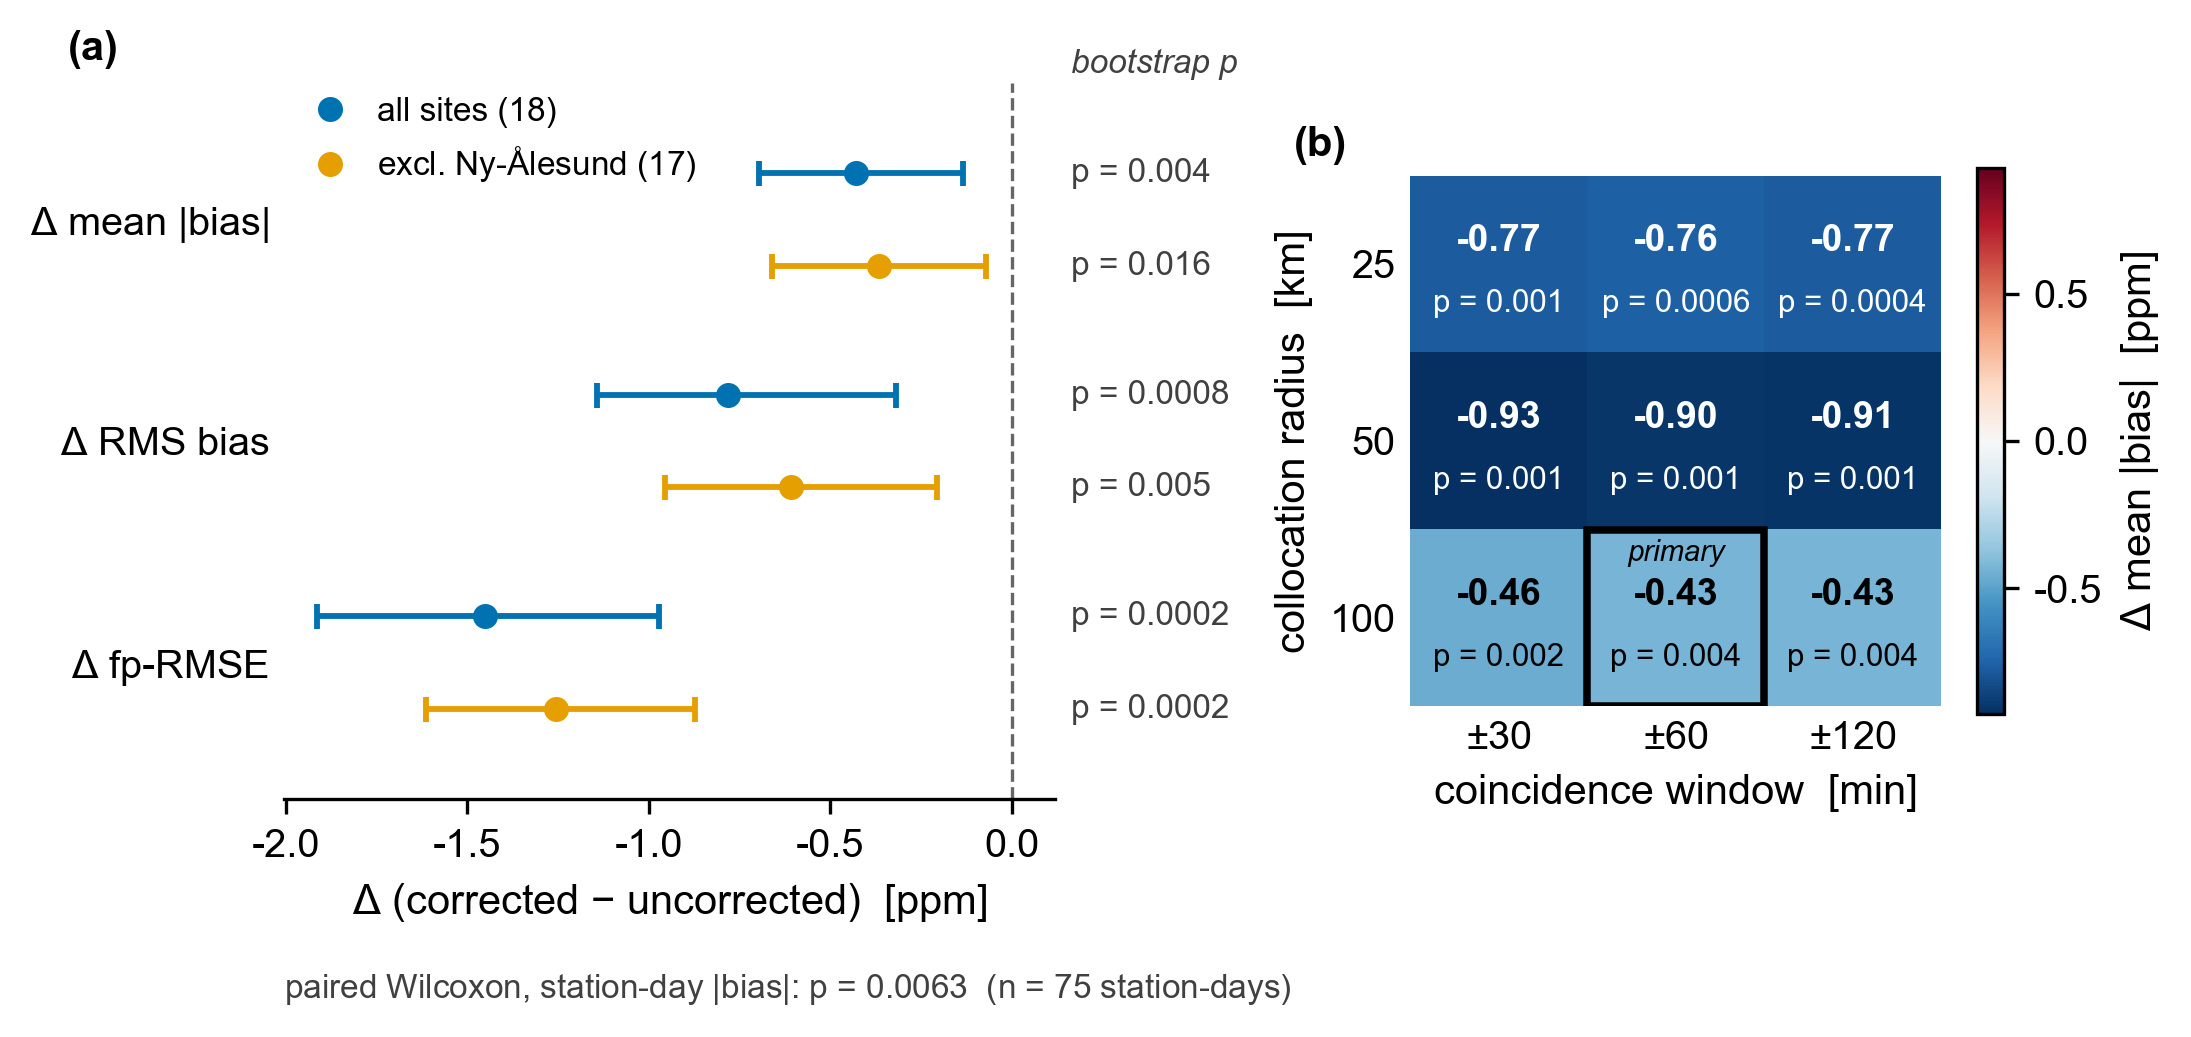
\includegraphics[width=0.8\textwidth]{figures/fig09_significance_robustness.png}
\caption{Significance and robustness of the TCCON validation: site-clustered bootstrap estimates with 95 \% confidence intervals for the change in station-day mean $|$bias$|$, RMS bias, and per-footprint RMSE (all sites and excluding Ny-Ålesund), and the change in mean $|$bias$|$ across collocation radius (25/50/100 km) × window (±30/60/120 min).}
\label{fig:tccon_significance_robustness}
\end{figure}





%% Generated by manuscript/scripts/make_manuscript_tables.py — do not hand-edit.
% Requires booktabs. Define in the preamble:
%   \newcommand{\xcobc}{$X_{\mathrm{CO2}}^{\mathrm{bc}}$}
%   \newcommand{\xcoraw}{$X_{\mathrm{CO2}}^{\mathrm{raw}}$}
\begin{table}[htbp]
\centering
\caption{Station-equal mean absolute bias to AK-harmonized TCCON (ppm): each station's footprint-weighted mean bias is taken in absolute value and averaged with equal station weights (18 stations). Best corrected value per row in bold.}
\label{tab:station-equal-bias}
\small
\begin{tabular}{lrrrr}
\specialrule{1.2pt}{0pt}{2pt}
QF & Before & DE & XGB & Ridge \\
\midrule
QF 0+1 & 0.98 & \textbf{0.73} & 0.74 & 0.83 \\
QF$\,$=$\,$0 & 0.60 & 0.60 & 0.63 & \textbf{0.58} \\
QF$\,$=$\,$1 & 1.36 & 0.82 & \textbf{0.80} & 0.96 \\
\specialrule{1.2pt}{2pt}{0pt}
\end{tabular}
\end{table}






\FloatBarrier